\documentclass[a4paper]{article}

\usepackage[english]{babel}
\usepackage[utf8]{inputenc}
\usepackage{amsmath}
\usepackage{graphicx}
\usepackage{hyperref}
\usepackage[colorinlistoftodos]{todonotes}
\usepackage{float}

\title{Methods of Data Analysis - Exercises 3 and 4}

\author{Lorenz Linhardt (a1247418), Raphael Mitsch (a1006529), Magdalena Schwarzl (a1209910)}

\date{\today}

\begin{document}
\maketitle

\section{Chapter 3: Advanced Regression Modelling}
\label{sec:regression}

\subsection{Chosen dataset}

We decided to choose the dataset "College", containing one numeric response variable and 17 predictors, one of them logical/boolean. A complete, color-coded scatterplot matrix portraying the covariance of every variable with every other variable is displayed in Figure \ref{fig:college_covComparison}. It's quite obvious that there are several correlations with high covariance values (shown in violet).

\begin{figure}[H]
\centering
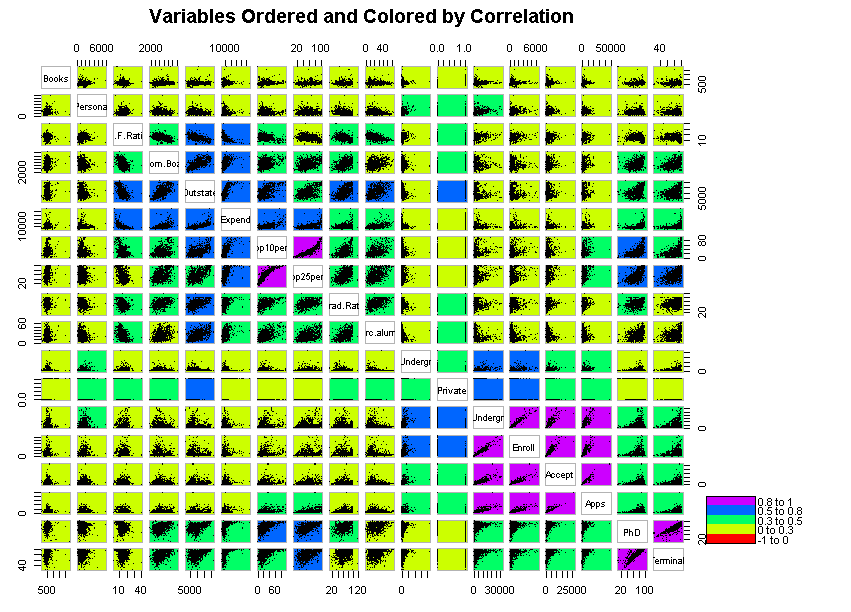
\includegraphics[width=1\textwidth]{spm_beforePreprocessing.png}
\caption{\label{fig:college_covComparison}Covariance matrices for all predictors in the College dataset.}
\end{figure}

\subsection{Preprocessing}
\label{sec:preprocessing}
\begin{figure}[H]
\centering
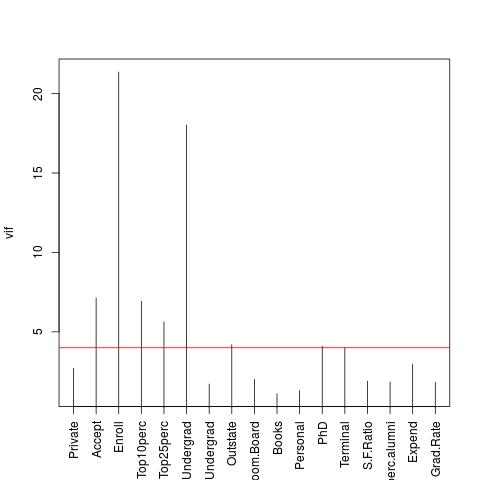
\includegraphics[width=0.5\textwidth]{vif_College.jpeg}
\caption{\label{fig:vifREG}Variance Inflation Factor for each column in the dataset.}
\end{figure}
%Magdalena
\label{desc:colinearity}After normalization of the data we removed columns with a Variance Inflation Factor bigger than 4 iteratively, as the vif is an indicator for colinearity (see Fig. \ref{fig:vifREG}). We used the R function \textit{vif()} for computation, deleted the column with the highest factor and called \textit{vif()} again until all values were smaller than 4.

The resulting set of predictors after the removal of said columns can be seen in Figure \ref{fig:college_covComparison_afterPreproc}.

\begin{figure}[H]
\centering
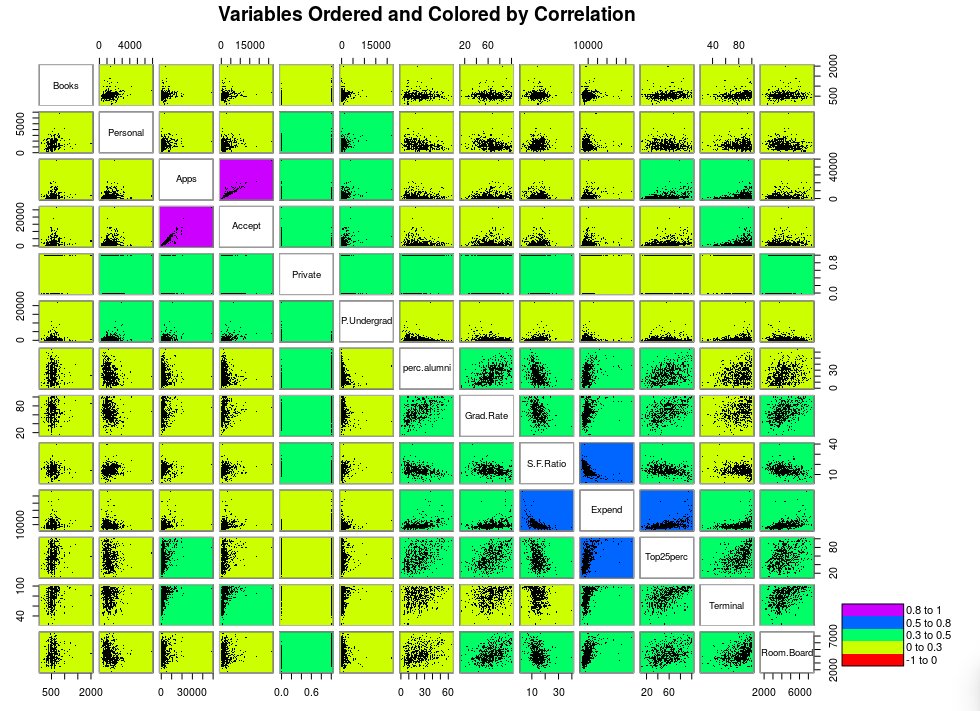
\includegraphics[width=0.9\textwidth]{covarianceMatrix.png}
\caption{\label{fig:college_covComparison_afterPreproc}Covariance matrices for predictors remaining in the College dataset after preprocessing.}
\end{figure}

We then split the data into a training (75\%) and a test (25\%) set. For both sets we create two different versions, one including outliers (used for the robust regression later) and one not including outliers. We decided to remove all instances with more than 2000 Apps as outliers (Fig. \ref{fig:lmAll} and \ref{fig:lmAllNoOulier} show the diagnostic plots of a linear regression model using the whole data set (training and testing) to show the effect of removing outliers).

\begin{figure}[H]
	\centering
	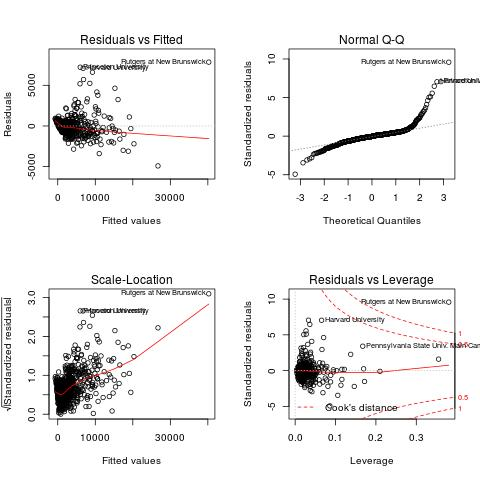
\includegraphics[width=0.6\textwidth]{lm_outlier.jpg}
	\caption{\label{fig:lmAll}Diagnostic plots of a linear regression model on the whole data set (test and training before cleaning). Absolute residual value increases with increasing x (Apps), distribution is not normal, homoscedasticity not given - variance increases by increasing x (Apps), multiple data points with high leverage and high residual value (e.g. Brunswick). Compare to Fig.  \ref{fig:lmAllNoOulier}}
\end{figure}

\begin{figure}[H]
	\centering
	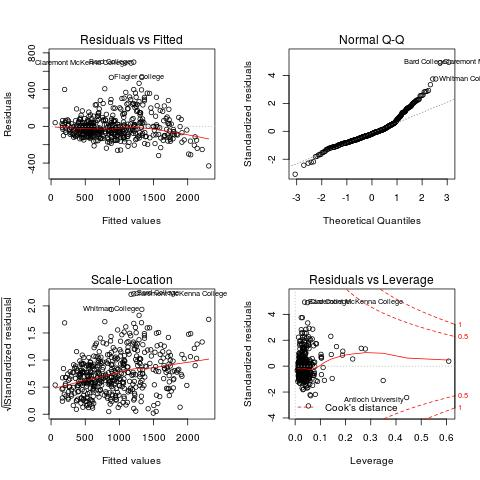
\includegraphics[width=0.6\textwidth]{lm_NOoutlier.jpg}
	\caption{\label{fig:lmAllNoOulier}Diagnostic plots of a linear regression model on the whole College data set (test and training set) NOT including outliers. Compared to Fig. \ref{fig:lmAll} residuals show a better distribution now.}
\end{figure}

The training set is split into $k = 10$ buckets used for cross validation in the training phase (see \it{CV.R}\rm).

\subsection{Test of Model Assumptions}
%Raphi
We tested for the following assumptions required by some of the methods we used: 
\begin{itemize}
  \item Homoscedasticity,
  \item independence and
  \item normality of errors.
\end{itemize}

\begin{figure}[H]
	\centering
	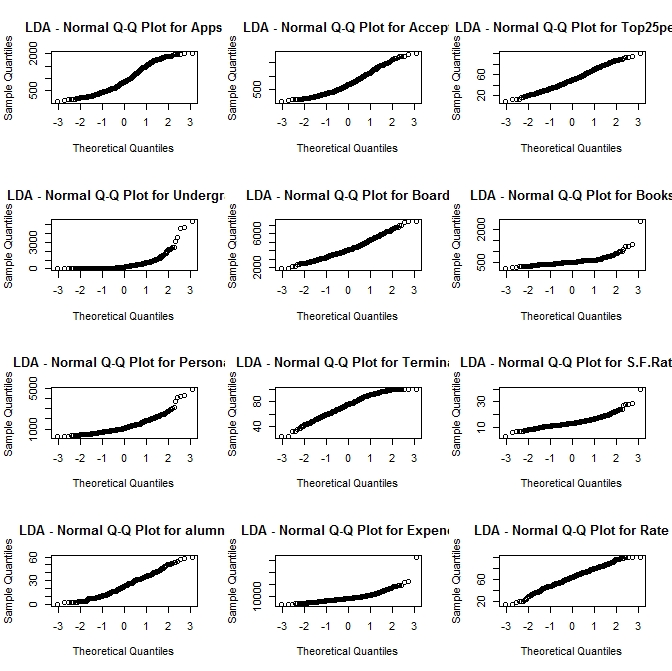
\includegraphics[width=0.6\textwidth]{qqPlots.jpg}
	\caption{\label{fig:qqPlots_regression}QQ plots for all numerical variables. None of the examined predictors follows the normal distribution.}
\end{figure}

\begin{figure}[H]
	\centering
	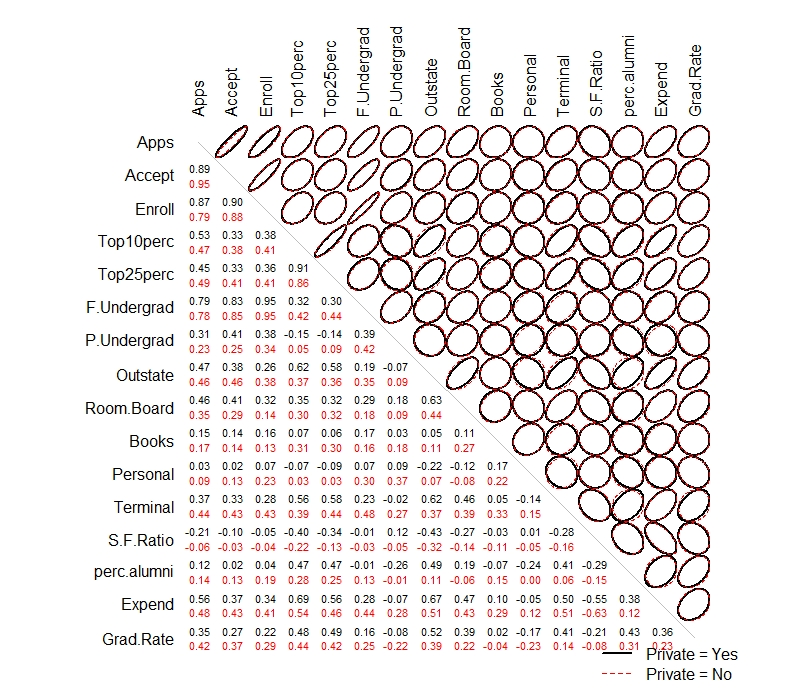
\includegraphics[width=0.75\textwidth]{covarianceComparison.jpg}
	\caption{\label{fig:covariance_regression}Comparison of covariance matrices between private and public universities. There is almost no difference in covariance between private and public universities.}
\end{figure}

We used the Breusch-Pagan test against \emph{heteroscedasticity}, which yielded a p-value of $4.355 \cdot 10^{-7}$ - low enough to reject $H_0$ (that the data is homoscedastic).

Next, we examined the normality of the data by (1) applying the Shapiro-Wilk normality test, which - assuming a significance level of $0.05$ - rejected $H_0$ (assumption of normality of errors)  for all variables. To confirm this, we took a look at the qq-plots for all variables (see Figure \ref{fig:qqPlots_regression}). While none of the examined predictors follows the normal distribution exactly, some of them approximate it rather closely.

For a discussion of how (in-)dependent the predictors are, see the beginning of Section \ref{desc:colinearity}.

Additionally, we were interested in whether or not the university being a private one had an influence on any of the other predictors - so we compared the covariance matrices of private and public universities, the result can be seen in Figure \ref{fig:covariance_regression}. Based on the aforementioned plot we concluded that there is no difference in the correlation between different predictors based on a university being private or public.

\subsection{Applied Models}
All of the following (except robust regression) have been computed using a cleaned version of the College data set (see Sec. \ref{sec:preprocessing} without outliers).

\subsubsection{Linear Regression}
% Magdalena
This first tests have been done separately from the cross validation (see file \emph{linearRegression.R}) and use the whole training data set omitting outliers.
At first we built a model using all columns not deleted in the pre processing ($R^2$ of 0.9074). In the summary we found out that many of the columns could be removed as they were not significant (e.g. Private, P.Undergrad,Room.Board,..). The model with less predictors performed similar to the full model ($R^2 = 0.907$). Removing also columns with low significance ($> 0.001$) resulted in $R^2 = 0.9018$. To decide whether the reduced model can be used, we did an analysis of variance test comparing the full with the reduced model (p-value = 0.9285) and the full with the most reduced one (p-value = 0.002979). The first test was not significant, allowing us to keep the null hypothesis and use the smaller model, however we could not use the fully reduced model as the second test was significant (assuming a confidence interval of 95\%).

\begin{figure}[H]
	\centering
	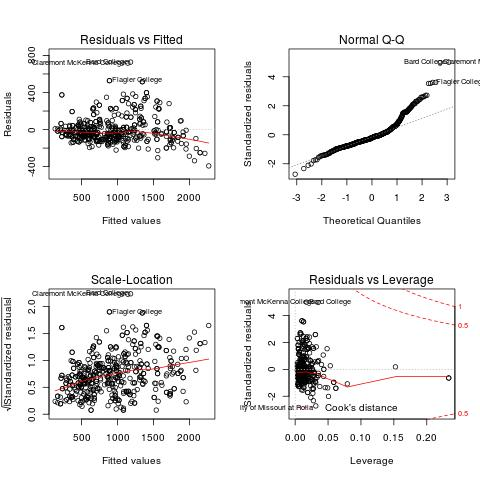
\includegraphics[width=0.75\textwidth]{lm_reduced.jpg}
	\caption{\label{fig:linReg}Linear regression with reduced data set (less columns). The plot is similar to Fig. \ref{fig:lmAllNoOulier} as only insignificant (using summary of lm object in R, which tests this using a T-Test in the last column) columns have been removed. Still - the distribution of the residuals is not perfectly gaussian.}
\end{figure}

\subsubsection{Cubic Splines}
%Raphi
Being a regression smoother (e.g. accessing local information only, without making any assumptions about underlying factors), cubic spline smoothing is susceptible for the curse of dimensionality. Nonetheless we applied it using the \texttt{gam()} function.
Since cubic splines are not able to cope with non-numeric data, we converted the logical values of the predictor 'Private' to numeric values (false to 0, true to 1). This and the number of dimensions give rise to the assumption that cubic splines won't perform well on this dataset.

\subsubsection{K-NN}
%Lorenz
%curse of dimensionality, plot

As we do not have too many columns left after preprocessing, we can also apply the k-nearest-neighbor algorithm that would be sensitive to high dimensional data, as it strongly depends on a distance measure and is thus susceptible to the curse of dimensionality. Other problems that could negatively influence the performance of this algorithm, such as missing values or highly correlated features are either taken care of in the preprocessing, or do not occur in our dataset.

Luckily there are no nominal attributes with more than two levels in the dataset, as we would have had to convert them to multiple binary attributes to make use of them with k-nn, since it usually does not make sense to have different values of an (unordered) nominal attribute to have different distances in terms of the k-nn algorithm.

We used the k-nn regression implementation provided by the \textit{FNN} library. Therefore, we had to convert the binary factor, that is the column 'Private', to a numerical dimension, containing the integers 0 and 1. We also normalized all numerical attributes to the range of 0 to 1 to avoid giving some attributes higher importance. 

As can be seen in figure~\ref{fig:knnReg}, we tuned the neighborhood-size on the training set using the $R^2$ of the result of 10-fold cross-validation. It seems that local structures are quite important in this dataset, as a k of 4 appears to be optimal. 
\begin{figure}[H]
	\centering
	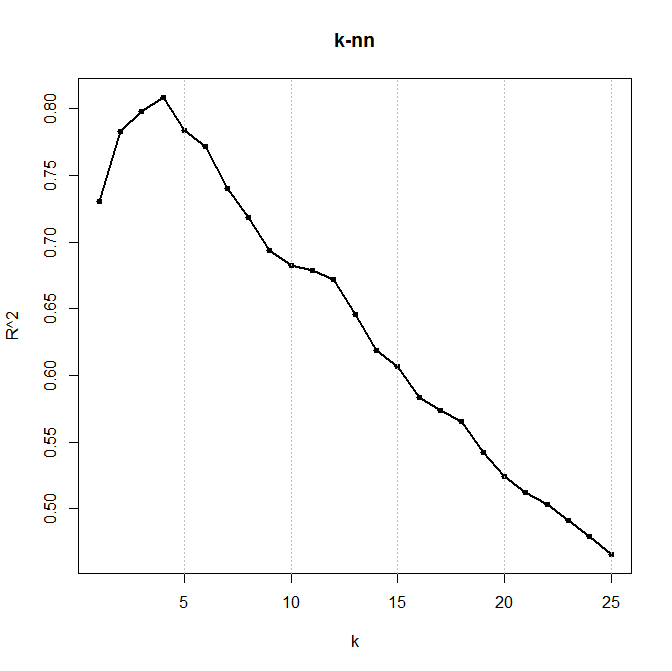
\includegraphics[width=0.75\textwidth]{kNNRegr_k-r2.png}
	\caption{\label{fig:knnReg} The neighborhood size k against the $R^2$ of the result.
    }
\end{figure}

\subsubsection{Non-linear Regression}
Here we again use the data set including all columns not reduced in the pre processing with removed outliers to build the models.

%Magdalena
\subsubsection{Box Cox transformation}

  \begin{figure}[H]
  	\centering
  	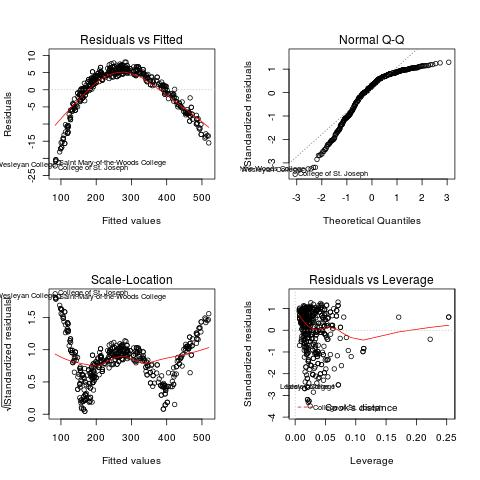
\includegraphics[width=0.75\textwidth]{boxcox.jpg}
  	\caption{\label{fig:boxcox} Results of Box Cox transformed linear model using the full outlier reduced training set without cross validation. The distribution of the residuals is obviously not normal. Compare to Figure \ref{fig:logTransform}.
      }
  \end{figure}

% We applied a box-cox transformation using the training set which resulted in a $R^2$ of 0.9968 for the whole training data set (no cross validation). Fig. \ref{fig:boxcox} shows the results.
% \subsubsubsection{log}
\textbf{Logarithmic Transformation} We also applied a logarithmic transformation using the training set which yielded a result displayed in Fig. \ref{fig:logTransform}.
 \begin{figure}[H]
 	\centering
 	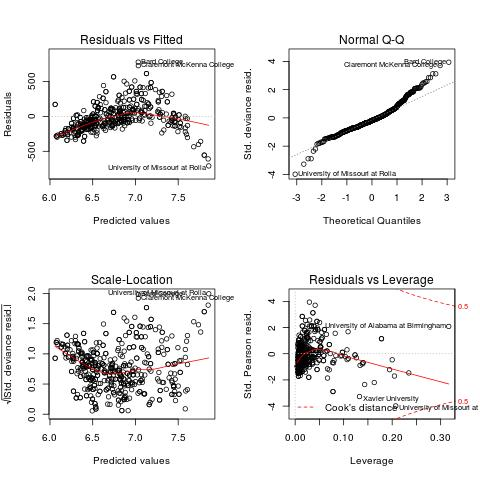
\includegraphics[width=0.75\textwidth]{logTransform.jpg}
 	\caption{\label{fig:logTransform}Transforming the response variable logarithmic and building a linear model on the complete outlier removed training set.}
 \end{figure}

\subsubsection{Robust Regression}
%Lorenz
As the dataset contains some outlying observations, we also applied robust regression methods. We trained robust methods once on the original data, and as comparison once on the set cleaned of outliers. 
We used the robust M-estimator with bisquare- and Huber-weight and also tried the LTS-estimator. 

On this dataset it worked best to use the Huber-weight, which has an objective function that is a compromise between the more rapidly increasing least squares and the bisquare function that is leveling off eventually.

Also, applying the robust methods on the data including outliers leads to better results, which could indicate that our removal of outliers in the preprocessing was too strict or simply that weighting the effect of outliers is more effective than just removing them.

\subsubsection{LOESS}
%Magdalena 
 Testing on the whole training data with removed outliers, we had difficulties in finding an implementation that supports more than 4 columns for the model building. We found \textit{locfit}, which does not restrict the formula to less than 4 predictors. However we could not use all columns due to limited resources (memory and time). As we did not find a way to decide for the best columns for LOESS specifically, we used the ones significant for linear regression. We used a tricubic kernel and a neighborhood of 20\%, a local polynomial of degree 1 gave the best performance on the test data set including outliers (see Fig. \ref{fig:loess}).

 \begin{figure}[H]
 	\centering
 	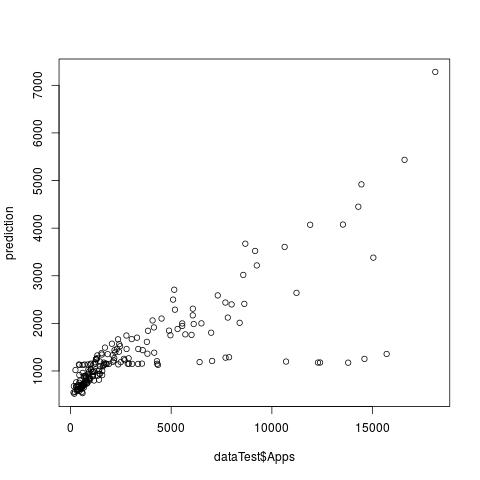
\includegraphics[width=0.6\textwidth]{loess.jpeg}
 	\caption{\label{fig:loess} True vs. predicted value of the test set including outliers using the loess model computed on the full training set without outliers (no cross validation; training set used.)}
 \end{figure}

 \subsubsection{Regression Tree}
%Raphi
We applied R's \texttt{rpart()} method on the data, hoping the regression tree would be able to cope with the non-normality we detected in our data (since it does not assume the presence of any kind of distributions - or linearity). 
We post-pruned our tree to avoid overfitting due to too complex tree structures, but didn't pre-prune in order to avoid premature pruning steps.

See Fig. \ref{fig:reg_tree_pruned} for the pruned decision tree.

 \begin{figure}[H]
 	\centering
 	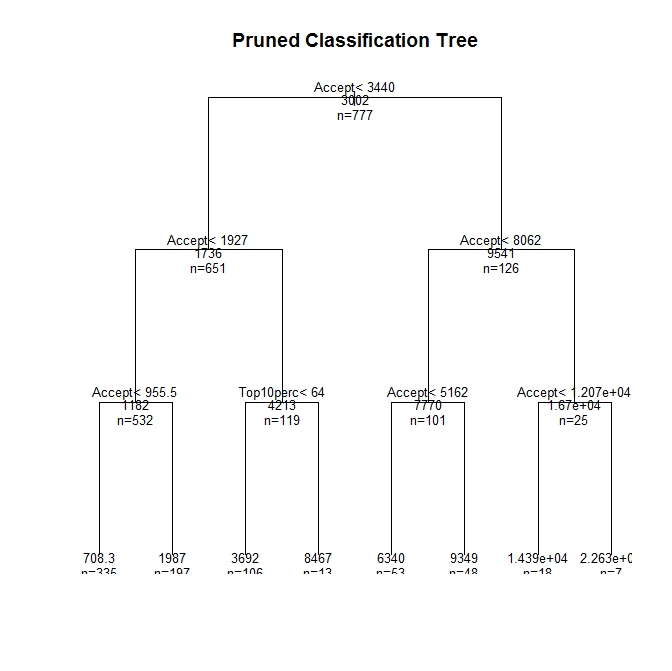
\includegraphics[width=0.6\textwidth]{regressionTree_pruned.jpg}
 	\caption{\label{fig:reg_tree_pruned} Pruned regression tree for the College dataset. Note that the acceptance rate is almost exclusively used.}
 \end{figure}
 
% assumes normality of response?
% http://alumni.media.mit.edu/~tpminka/courses/36-350.2001/lectures/day20/
% no assumptions?
% http://support.sas.com/resources/papers/proceedings13/089-2013.pdf

% post pruning “better”
% cost-complexity criterion used by rpart

 \subsection{Model Evaluation and Selection}
% Magdalena, Raphi, Lorenz
% TODO: training on no-outliers (except robust), and predicting on with-outliers

 We decided to use 75\% of the original dataset as training data and 25\% as test set. Model selection was done by comparing the RMSE of the cross-validation of all our models on the training set. To avoid overly optimistic expectations of the performance of our final model, possibly introduced through overfitting in the model selection phase, we re-trained the seemingly most accurate model on the whole training set and estimated its generalization ability on the hold-out test set.

We trained our models (except robust regression) on the dataset without outliers and tested them on the dataset including outliers. Our rationale behind this decision is that we do not want to skew out models through outliers, but we would like to know how well they do on \textit{any} incoming data.

We chose the RMSE as measure of model quality, as it is a quite common measure and can be applied to all kinds of models.

\begin{table}[H]
\begin{tabular}{|l|r|}
\hline
Method & RMSE \\\hline
 k-nn &  4812.059\\
 Cubic Spline & 1525.873 \\
 Linear Regression & 1516.662\\
 LOESS & 21570.03 \\
 Regression Tree & 3938.292 \\
 \textbf{Robust M-Estimator with Huber-Weight} & \textbf{1208.846} \\
 Robust M-Estimator with Bisquare-Weight &  1336.591\\
 LTS-FIT* &  1458.397\\
 Robust M-Estimator with Huber-Weight* & 1530.724 \\
 Robust M-Estimator with Bisquare-Weight* &  1559.480\\
 LTS-FIT* &  1554.008\\
 Box-Cox transformation & 3889.404 \\
 Log transformation & 4797.358 \\
\hline
\end{tabular}
\caption{Results of the applied methods, evaluated via the RMSE. The methods marked with a * are trained on the training set inclusive outliers. For all others, outliers have been removed for training. }
\end{table}

We evaluated the seemingly best performing model (Robust M-estimator with Hubert weight) on the training set, resulting in an RMSE of 1144.666.

Another method that seemed to work well was k-nn without normalizing the predictors first (not listed in the table). The reason for this should be that the attributes having high values are more important for accurate prediction than the others. We could not verify that any high-valued attribute works particularly well in isolated tests though. 

\section{Chapter 4: Advanced Classification Modelling}
\label{sec:classification}

\subsection{Chosen dataset}

We chose the credit default dataset for classification purposes. The response variable is logical (default or not), while the predictors are:
\begin{itemize}
	\item \emph{student} (logical),
   	\item \emph{balance} (numerical) and
    \item \emph{income} (numerical).
\end{itemize}
While income and balance seem - intuitively - obviously helpful for predicting whether someone will default or not, a person's student status may or may not have any influence on the outcome.

This is a highly imbalanced dataset - $96.6\%$ of rows have $default = No$, only the remaining $0.34\%$ carry positive default values. For further elaboration on how this may influence the results see Section \ref{sec:Evaluation}.

\subsection{Preprocessing}
%Magdalena
We splitted the data into a training set (75\%) and created 10 stratified folds within this subset to perform for cross validation. The remaining 25\% are used to test our models later. 

\subsection{Test of Model assumptions}

Similarly to the regression part, we tested against the following assumptions required by some of the methods we used: 
\begin{itemize}
  \item Homoscedasticity,
  \item similarity of covariance matrices for both values of the response variable and
  \item normality of errors and
  \item whether being a student makes a significant difference.
\end{itemize}

\begin{figure}
	\centering
	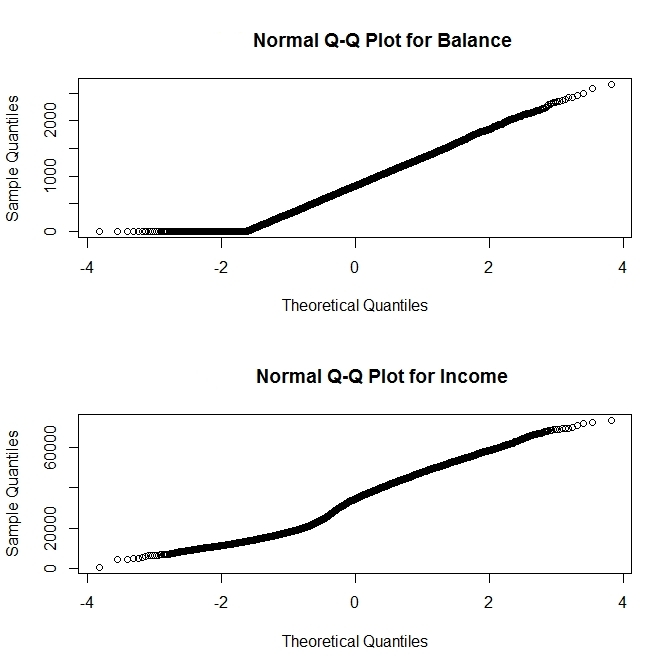
\includegraphics[width=0.6\textwidth]{qqPlots_classification.jpg}
	\caption{\label{fig:qqPlots_classification}QQ plots for both numerical variables in credit card default dataset. Neither can be assumed to follow a Gaussian distribution.}
\end{figure}

\begin{figure}
	\centering
	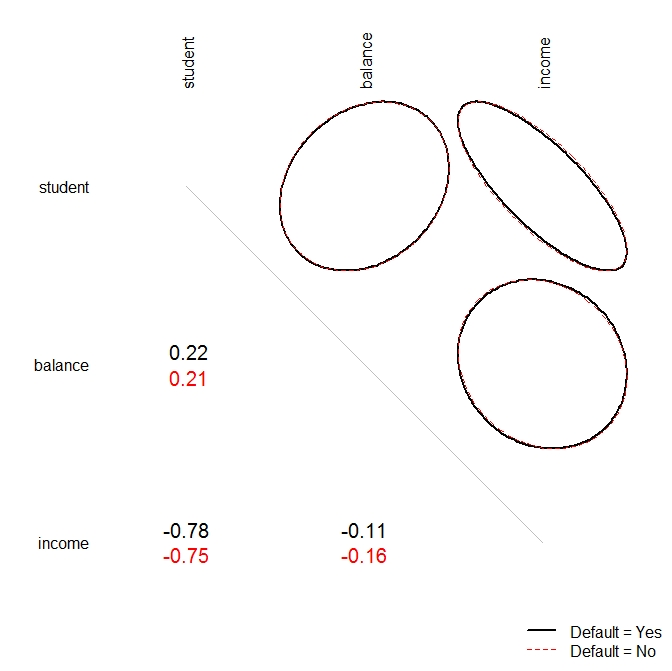
\includegraphics[width=0.65\textwidth]{covarianceComparison_classification.jpg}
	\caption{\label{fig:covariance_classification}Comparison of covariance matrices between subjects having defaulted or not. There hardly any difference in covariance between the two response classes (\emph{default = yes} or \emph{default = no}).}
\end{figure}

We used the Breusch-Pagan test against \emph{heteroscedasticity}, which yielded a p-value of $2.2 \cdot 10^{-16}$ - suspiciously close to zero\footnote{See here: \href{http://stackoverflow.com/questions/6970705/why-cant-i-get-a-p-value-smaller-than-2-2e-16}{P-values in R smaller than $2.2\cdot10^{-16}$}}. To be able to execute the Breusch-Pagan test at all we had to convert the response variable, which was stored as a factor, to a logical variable - the BP-test can't seem to scope with non-numerical data (any hints are appreciated).
Conclusively, we couldn't judge with confidence whether our data is hetero- or homoscedastic.

Next, we examined the normality of the data by (1) applying the Shapiro-Wilk normality test, which (for a significance level of 0.05) rejected $H_0$ for all variables. To confirm this, we took a look at the qq-plots for all variables (see Figure \ref{fig:qqPlots_classification}). While income doesn't seem to follow the normal distribution exactly, balance actually seems like it would, if it wasn't for of lot of datasets with with a balance of 0.

Additionally, we were interested in whether or not the covariance matrices differ between the response groups (default, no default). The result of this comparison can be seen in Figure \ref{fig:covariance_classification}. Based on the aforementioned plot we concluded that there is no difference in the covariance matrices in the two response classes.


\subsection{Applied Models}
% Magdalena, Raphi, Lorenz
Again we aimed to apply the whole range of models introduced in the lecture.

\subsubsection{Logistic Regression}
Logistic regression counters problems with non-normality and heteroscedasticity, which arise e.g. in classification with dichotomous response variables (such as default in our case). Logistic regression applies a transformation function - logit, probit, etc. - on the regression formula to improve results.

We used logistic regression with the default parameters and specified the binomial distribution family as distribution family to follow.
% https://en.wikipedia.org/wiki/Predictive_analytics#Classification_and_regression_trees
\subsubsection{K-NN}
%curse of dimensionality, unbalanced classes, k-error rate(plot), bool->1,0, library

To use this implementation we used the \textit{class} library, and again had to transform the boolean factor into a numeric vector, containing the integers 0 and 1 for 'no' and 'yes' respectively and to normalize the data values in each column to the range between 0 and 1.

As can be seen in figure~\ref{fig:kNNClass}, we again tuned the parameter k on the training set via cross-validation, leading to a seemingly best value of k=1 when considering balanced accuracy. As evaluation measure we applied balanced accuracy, to address the imbalanced nature of this dataset. To detect possible overfitting through parameter-tuning, the classification performance can eventually be verified on the test set. 

 \begin{figure}[H]
 	\centering
 	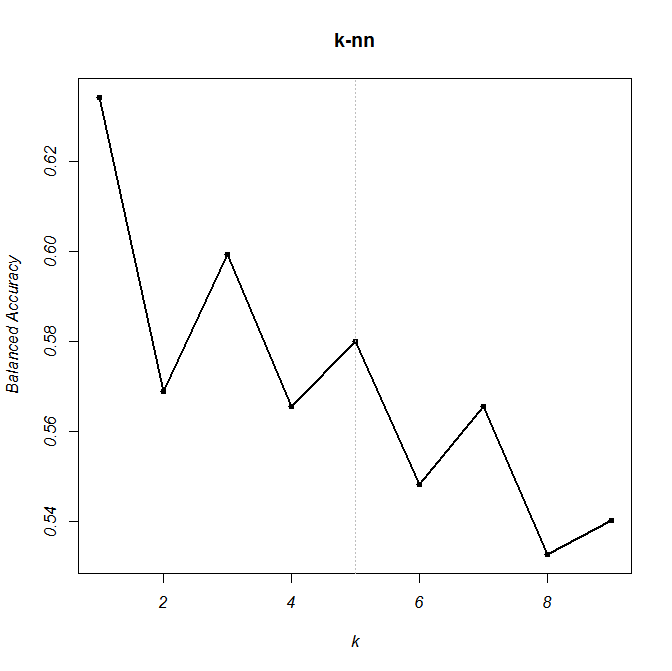
\includegraphics[width=0.6\textwidth]{kNNClass.png}
 	\caption{\label{fig:kNNClass} A k of 7 seems to be the optimal choice if the balanced accuracy is the chosen criterion.}
 \end{figure}

\subsubsection{Naive Bayes}
Naive Bayes assumes the independence of attributes given the class. We covered this assumption in the initial tests, yielding the result that this assumption is true.

Since we have only two class values, and sufficient examples of both classes, we decided not to use Laplace-correction.

As prior probabilities the class proportions are used since we do not have additional knowledge that would enable us to infer more sophisticated priors.

Initially we used the implementation of the \textit{e1071} library, which assumes a Gaussian distribution of predictors. As is not valid based on our previous tests, we switched to the implementation of the \textit{klaR} package, which does not rely on this assumption.


\subsubsection{Decision Tree}
%Magdalena
 \begin{figure}[H]
 	\centering
 	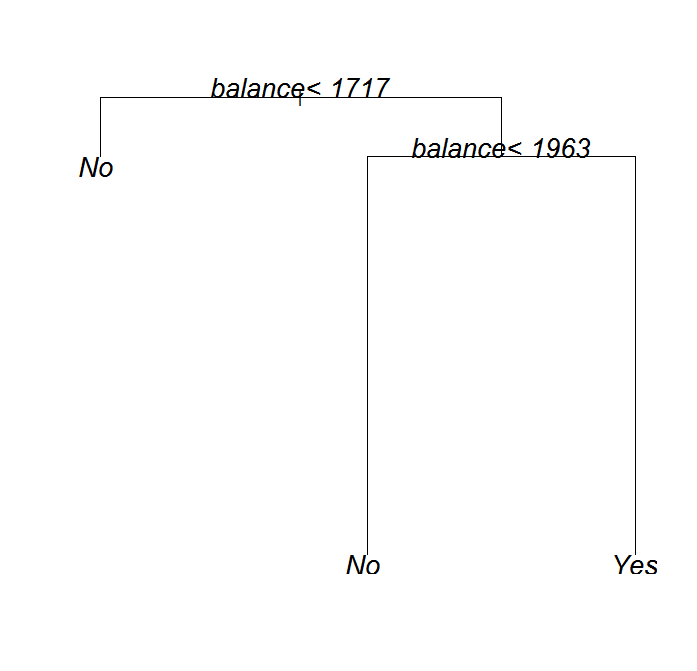
\includegraphics[width=0.6\textwidth]{decisionTree.png}
 	\caption{\label{fig:decisionTree} Left unpruned tree, right pruned tree.}
 \end{figure}

We build a first tree using the whole 75\% training set created in the pre processing script setting $cp = 0.000001$ (cost-complexity criterion). This results in a very complex tree, as the stop criterion is very low (Fig. \ref{fig:decisionTree} left). We later prune this tree with the cp value giving a minimal error using post pruning, as this usually is better (pre pruning can result in stopping too early). The pruned tree is shown in Fig. \ref{fig:decisionTree} on the left. 
The pruned tree has a sensitivity of 45.88 and a specifity of  99.31 indicating a high number of false negatives and low number of false positives.
% this is the confusion matrix:\\
% Sensitivity:  45.88\\
% Specifity  99.31"\\
%        True: 0 True: 1     \\
% Pred: 0    7195     138 7333\\
%Pred: 1      50     117  167\\
%           7245     255 7500\\
 
\subsubsection{Random Forest}
%Raphi
%Random forest
To counter the inherent problems occurring when analyzing a highly imbalanced dataset, we used an implementation of a random forest - a bagging approach. This is supposed to balance out the bias towards the more frequent class that is often encountered in singular models. A random forest basically aggregates (e.g. averages) the results of many decision trees and classifies based on the final, aggregated model.

We limited our random forest to 250 trees due to performance reasons.
%Random forest
\subsubsection{LDA, QDA}%wobei zumindes naive bayes glaub ich auch ein LDA ist 
LDA tries to find the projection that minimizes in-group and maximizes the between-group variance. LDA makes the assumption that the data is homoscedastic, while QDA accounts for heteroscedasticity. While we couldn't reasonably interpret able use the Breusch-Pagan test, the fact that the covariance matrices of both groups are highly similar at least suggests that the assumption of homoscedasticity is given.

% kopiert von 
% https://en.wikipedia.org/wiki/Linear_discriminant_analysis
\subsection{Evaluation}
\label{sec:Evaluation}
% Magdalena, Raphi, Lorenz
% model selection on testset vie CV, evaluation of final model on hold-out test set, roc/confusion matrix, unbalanced class -> bad for small class
For model selection we applied the same approach as for the regression problem, in terms of data splitting and the general procedure. The only difference lies in the evaluation measure of the classification results. For this we chose the AUC.

\begin{table}[H]
\begin{tabular}{|l|r|}
\hline
Method & AUC \\\hline
Decision tree & 0.777\\
\textbf{LDA} & \textbf{0.949}\\
\textbf{Logistic Regression} & \textbf{0.949}\\
Naive Bayes& 0.944\\
\textbf{QDA}& \textbf{0.949}\\
k-nn& 0.5\\
Random forest& 0.854\\
\hline
\end{tabular}
\caption{Results of the applied methods, evaluated via the AUC.}
\end{table}

The ROC curves for all models are plotted in Figure \ref{fig:roc_classification}. 
\begin{figure}[H]
	\centering

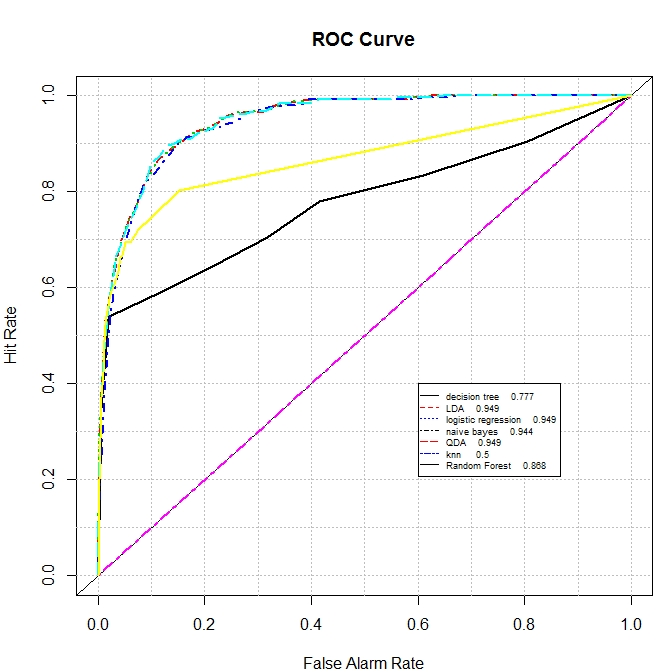
\includegraphics[width=0.8\textwidth]{ROC_classification.jpg}
 	\caption{\label{fig:roc_classification} ROC curves for all applied models.}
\end{figure}
 
Again, we verified the performance of the best models on the test set. Since the credit card debt default data set is a highly imbalanced one, we wanted to check if
\begin{itemize}
	\item (1) the proportion between true positive and false positive rates differs from
    \item (2) the proportion of true negative and false negative rates for varying cutoff rates.
\end{itemize}
I.e. we wanted to check if our model works properly and not just by declaring the vast majority as negative, which would still yield a acceptable overall accuracy. For this, we compared the ROC curves (1) and (2) for both of our selected models (LDA and logistic regression) as well as for the random forest approach, since bagging may alleviate problems with imbalanced datasets. This comparison can be seen in figure \ref{fig:tprfpr_tnrfnr_comparison}.

\begin{figure}[H]
	\centering
 	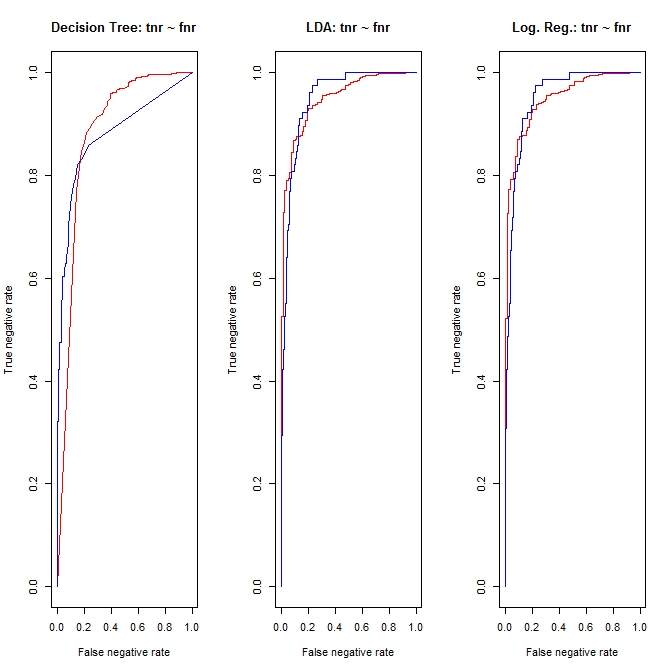
\includegraphics[width=0.6\textwidth]{tprfpr_tnrfnr_classification.jpg}
 	\caption{\label{fig:tprfpr_tnrfnr_comparison} Comparison between ROC curves for TPR vs. FPR (blue) and TNR vs. FNR (red). Almost no difference between the two curves for LDA and logistic regression; slightly better performance for TNR vs. FNR than for TPR vs. FPR for a random forest with $n = 250$.}
\end{figure}

LDA and logistic regression exhibit a highly similar distribution for both proportions, while random forest (overall not performing better than the other two models, so a simple bagging approach  doesn't seem to work that well here) seems to be better at correctly identifying negatives than positives.
 
We applied our two best-performing models - LDA and logistic regression - on the held-back test data set. The results are plotted in Figure \ref{fig:roc_classification_final}.

\begin{figure}[H]
	\centering
 	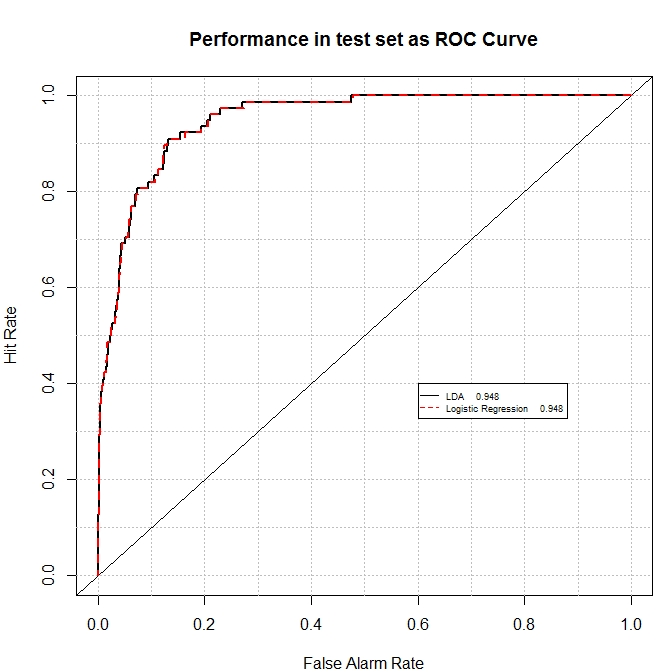
\includegraphics[width=0.8\textwidth]{ROC_classification_final.jpg}
 	\caption{\label{fig:roc_classification_final} ROC curves of the two best-performing models (LDA and logistic regression) on the final test set. Both curves look similar and give approximately the same AUC value}
\end{figure}
 
Another interesting phenomenon is that k-nn with k=1 results in a AUC of 0.5, meaning that it's not better than random guessing. This is surprising to us, since we even optimized the k on the training set, but we could not find the reason for this behavior.  

\end{document}